\documentclass[10pt,aspectratio=169]{ctexbeamer}
\usepackage{amsmath}
\usepackage{subfigure}
% \usepackage{xeCJK}
\usepackage[style=authortitle]{biblatex}


\usetheme{Madrid}
% \pgfdeclareimage[width=\paperwidth,height=\paperheight]{bg}{ecnu_background}
% \setbeamertemplate{background}{\pgfuseimage{bg}}
\setbeamertemplate{frametitle continuation}[from second]
\useinnertheme{rectangles}
\setbeamertemplate{theorems}[numbered] 
\usecolortheme[RGB={182,11,45}]{structure}
\usefonttheme{professionalfonts}
\logo{
\includegraphics[width=0.12\textwidth]{logo.png}}

%%%%%%%%%%%%%%%%%%%%%%%%%%%%%%%%%%%%%%%%%%%%%%%%%%%%%%%%%%%%%%%%%%%%%%%%%%%%%%%%
\title{数据可视化技术\, 论文分享}
\subtitle{TopKube: A Rank-Aware Data Cube for Real-Time Exploration of Spatiotemporal Data}
\author{蔡盛梁}
\institute{华东师范大学计算机科学与技术学院}
\date{2020 年 11 月 20 日}
\addbibresource{main.bib}

\begin{document}
\begin{frame}
    \titlepage
\end{frame}

\begin{frame}
    \begin{center}
        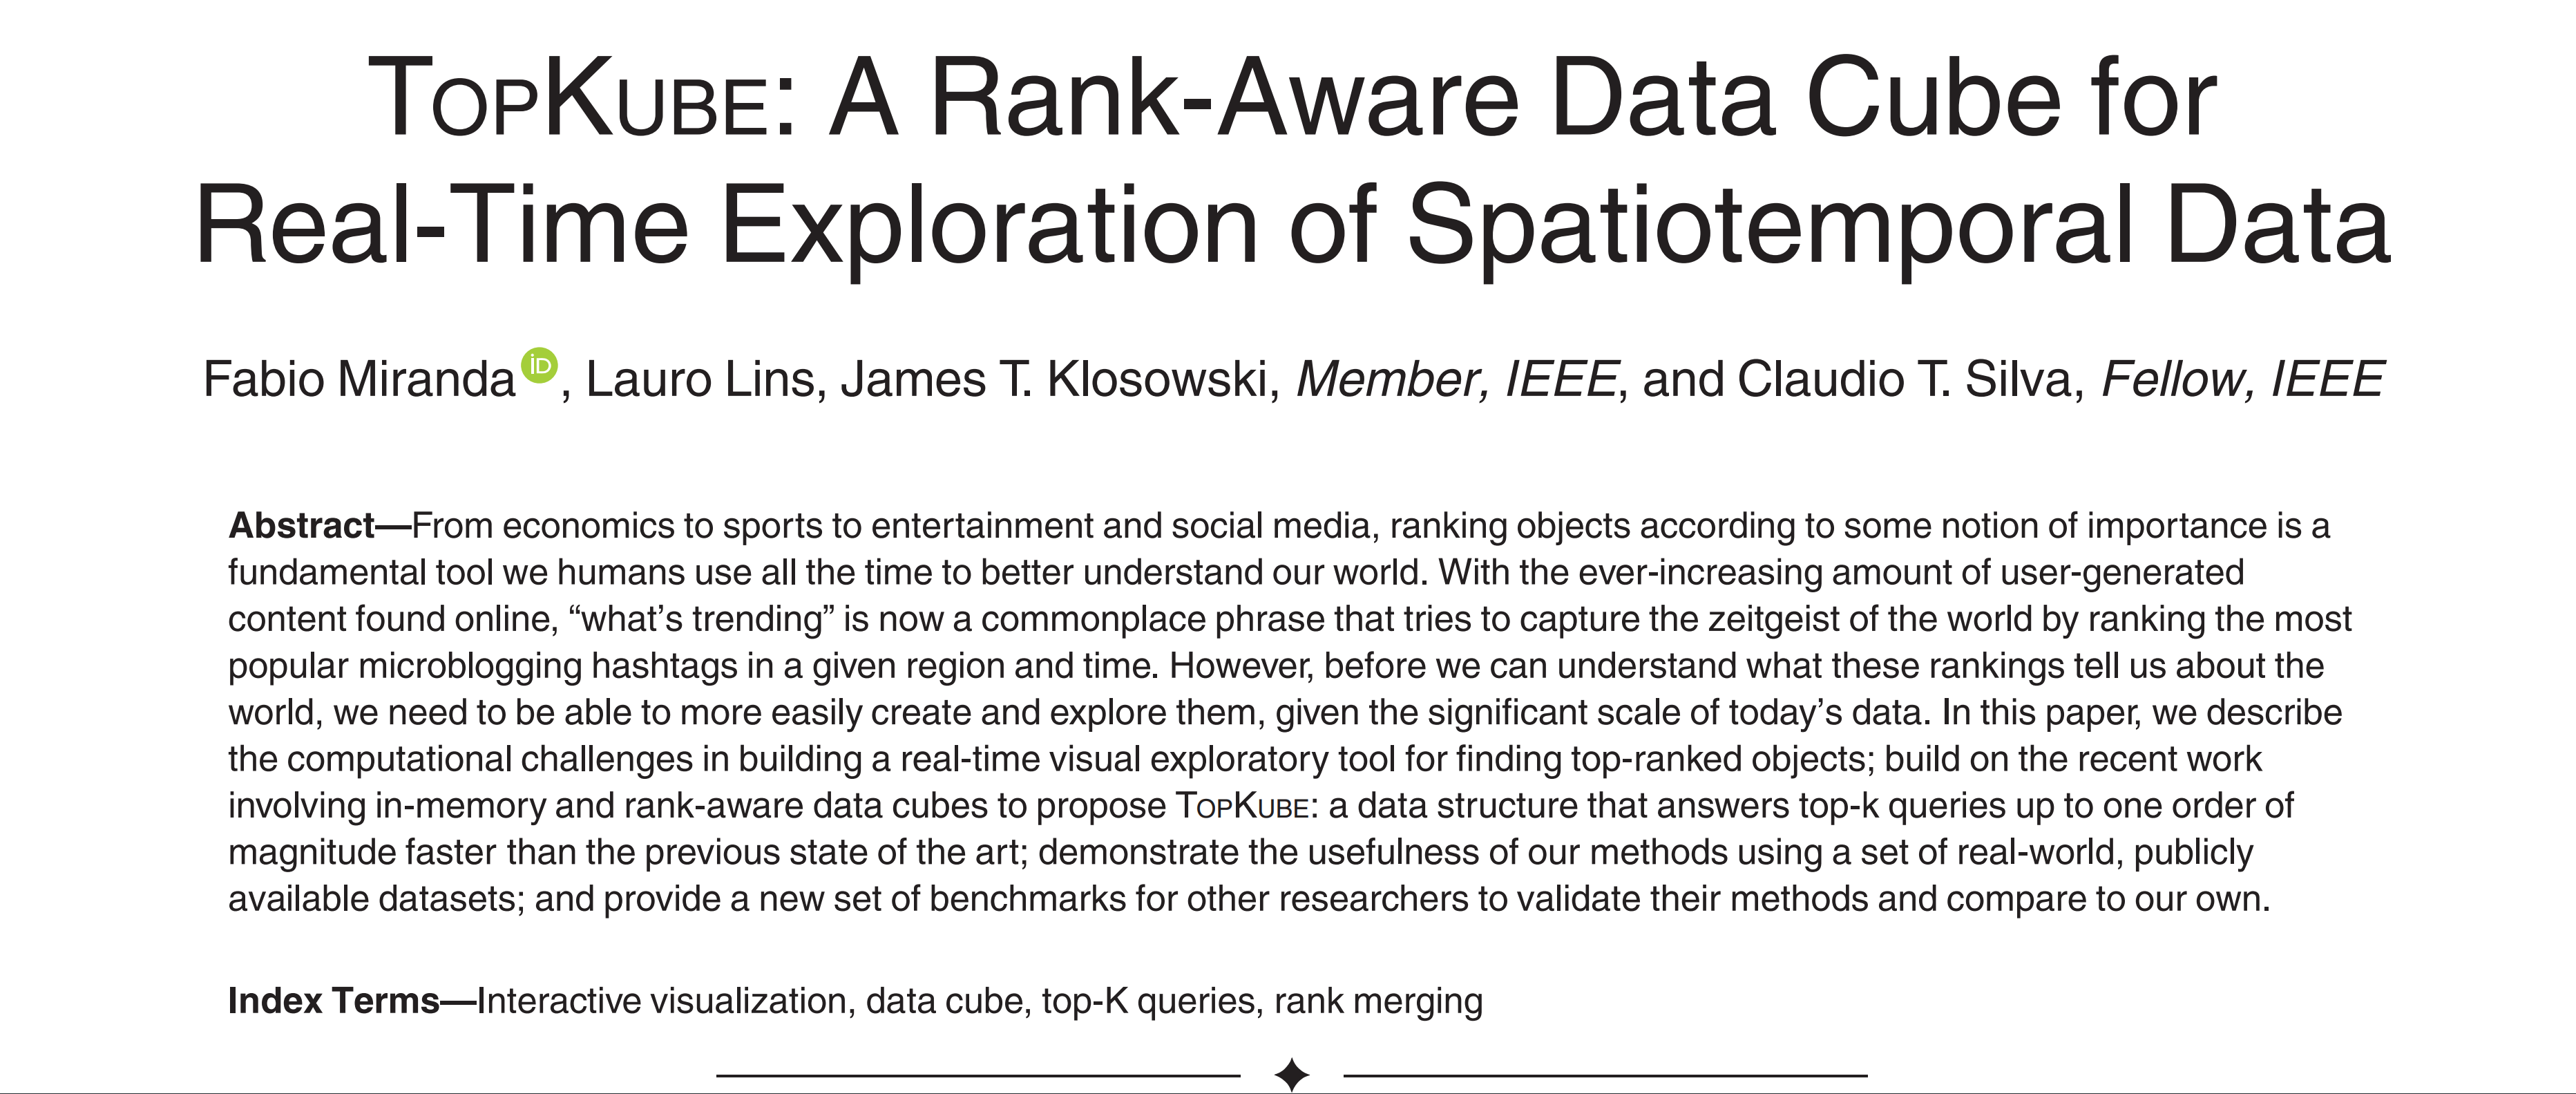
\includegraphics[width=.8\textwidth]{pic/paper.png}
    \end{center}
\end{frame}

\begin{frame}{背景\footcite{Miranda2018}}
    \begin{itemize}[<+->]
        \item 排序是人们日常生活中认识世界的重要方式。
        \item 如何处理时空数据排序问题变得重要。
        \item 交互式探索要求系统具有低时延。
        \item 相关工作没有关注查询前 $k$ 个最相关的结果。
    \end{itemize}
\end{frame}

\begin{frame}{数据立方体}
    \begin{itemize}[<+->]
        \item 数据立方体的概念首先在数据库领域中被提出。
        \item 对于若干维度,每个维度各取一个值,对各个维度的值都与指定的值相同的数据项组成了一个集合,返回关于集合中数据记录的聚合值。
        \item 预先计算并存储所有可能的维度值组合的聚合值。
    \end{itemize}
\end{frame}

\begin{frame}{NanoCubes\footcite{Lins2013}}
    \begin{columns}
        \begin{column}{.65\textwidth}
            \begin{itemize}[<+->]
                \item 按照维度进行分层,每个维度可以有内部的层次结构。
                \item 黑色连线代表维度内部不同层次的连接,而蓝色连线代表跨越维度的连接。
                \item 每一个内部节点对应于维度的一个取值,称为\textbf{箱}(bin)。
                \item 从根到叶子节点的路径视为在经过的维度选取了一组箱,这些不同维度选取的箱的组合称为\textbf{箱乘积}(product-bin)。
                \item 叶子节点存储箱乘积对应的数据集合的聚合值。
            \end{itemize}
        \end{column}

        \begin{column}{.35\textwidth}
            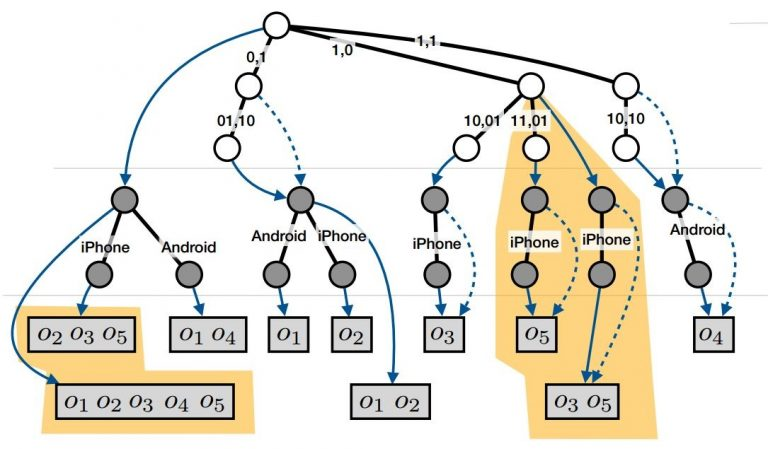
\includegraphics[width=\textwidth]{pic/nanocubes.jpg}
        \end{column}
    \end{columns}
\end{frame}

\begin{frame}{TopKube}
    \begin{columns}
        \begin{column}{.6\textwidth}
            在 Nanocubes 的叶子节点中,附加了 3 个数组:$q$, $v$, $\sigma$,以及一个聚合值:$\sum v$。
            \begin{itemize}
                \item $q$ 按照键本身的顺序存储键。
                \item $v$ 是 $q$ 中对应下标处键的测量值。
                \item $\sigma$ 是按照测量值从大到小排序的排名。
                \item $\sum v$ 是原有 Nanocubes 中存储的测量值。
            \end{itemize}
        \end{column}
        \begin{column}{.4\textwidth}
            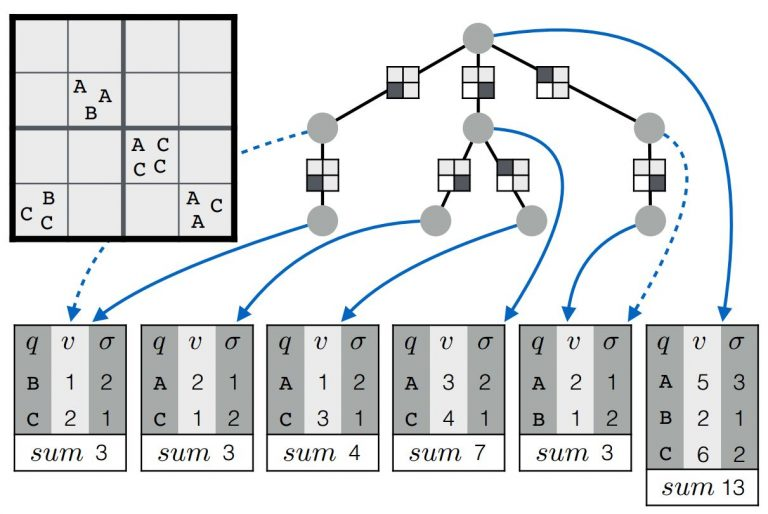
\includegraphics[width=\textwidth]{pic/topkube.jpg}
        \end{column}
    \end{columns}
\end{frame}

\begin{frame}{Top-k from Ranked Lists, TKR}
    \begin{columns}
        \begin{column}{.6\textwidth}
            \begin{itemize}[<+->]
                \item 实际的查询可能需要对多个箱乘积中的键的测量值之和进行排序。
                \item 这一问题称为从一些排序的数组中选取和前 $k$ 大的元素 (Top-k from Ranked Lists, TKR)。
                \item 针对这一问题,该论文提出三种算法。
            \end{itemize}
        \end{column}
        \begin{column}{.4\textwidth}
            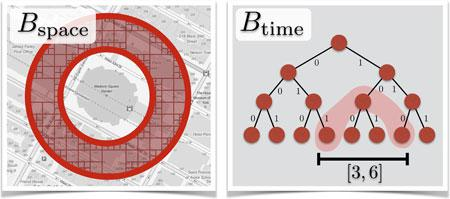
\includegraphics[width=\textwidth]{pic/query.jpg}
        \end{column}
    \end{columns}
\end{frame}

\begin{frame}{扫描算法 (Sweep Algorithm)}
    \begin{columns}
        \begin{column}{.3\textwidth}
            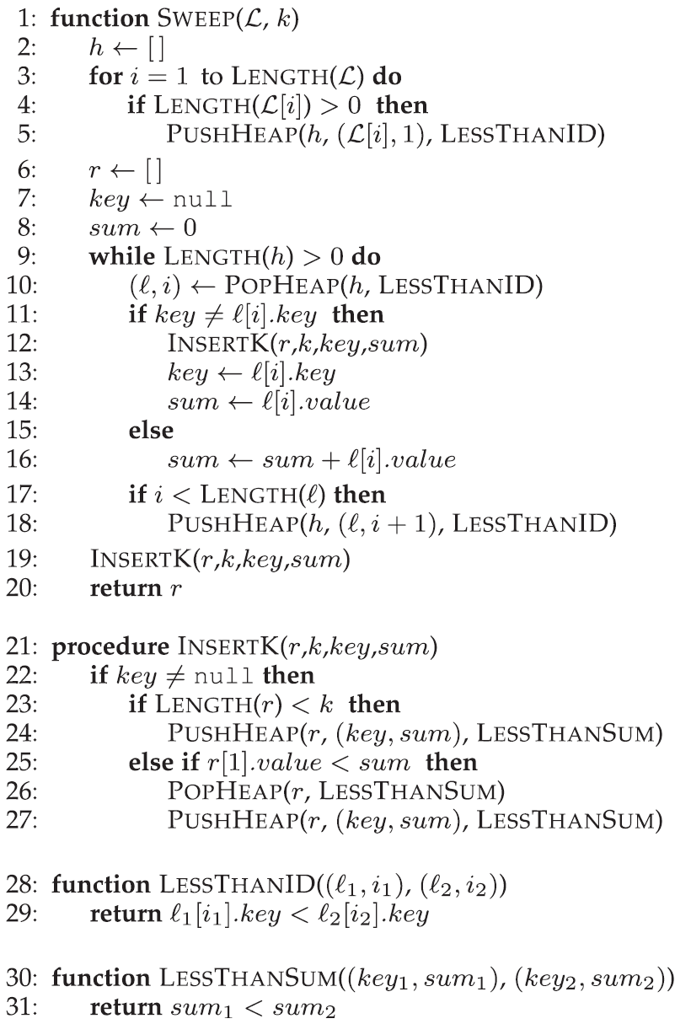
\includegraphics[width=\textwidth]{pic/sweep.png}
        \end{column}
        \begin{column}{.7\textwidth}\pause
            \begin{itemize}[<+->]
                \item 这一算法没有考虑排序信息,因此对于 Nanocubes 也适用。
                \item 维护两个最小堆。第一个堆存储每一个箱乘积中的当前最小键和对应的值,第二个堆维护已有的聚合值前 $k$ 大的键。
                \item 算法总时间复杂度为 $O(m \log m + N\log k + N\log m)$。
            \end{itemize}
        \end{column}
    \end{columns}
\end{frame}

\begin{frame}{阈值算法 (Threshold Algorithm)\footcite{FAGIN2003614}}
    \begin{columns}
        \begin{column}{.3\textwidth}
            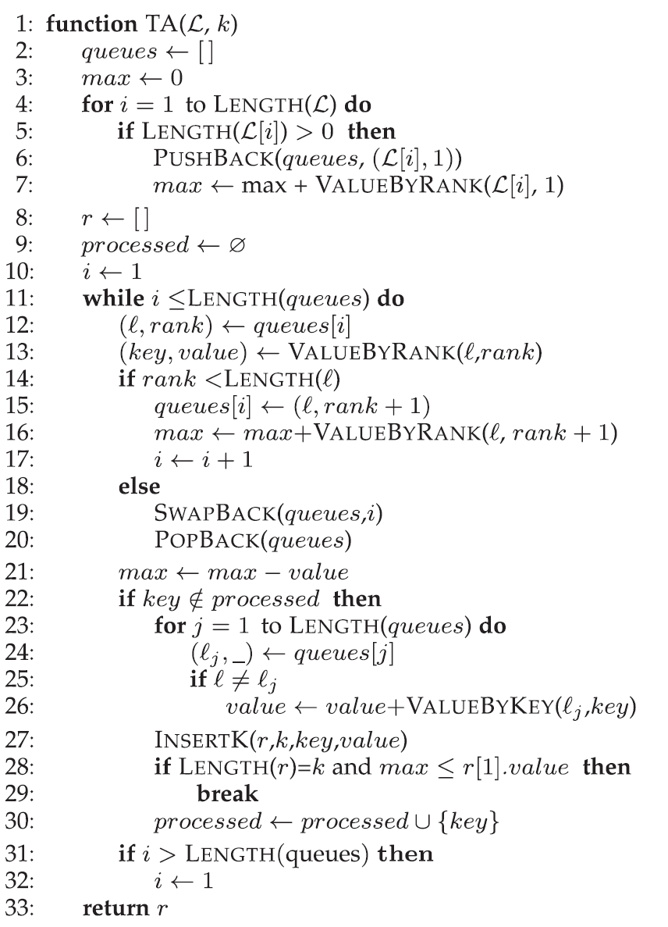
\includegraphics[width=\textwidth]{pic/ta.png}
        \end{column}
        \begin{column}{.7\textwidth}\pause
            \begin{itemize}[<+->]
                \item 计算机科学领域的一种常见算法。
                \item 维护一个队列和一个大小为 $k$ 的最小堆。
                \item 贪心选择 + 终止条件:当
                      \begin{enumerate}
                          \item 找到的键已经达到 $k$ 个;
                          \item 当前剩余的所有的箱乘积最大值的和小于已有的第 $k$ 大的结果。
                      \end{enumerate}
                \item 算法最坏的时间复杂度:$O(m + Nm + N \log k)$
            \end{itemize}
        \end{column}
    \end{columns}
\end{frame}

\begin{frame}{混合算法 (Hybrid Algorithm)}
    \begin{columns}
        \begin{column}{.3\textwidth}
            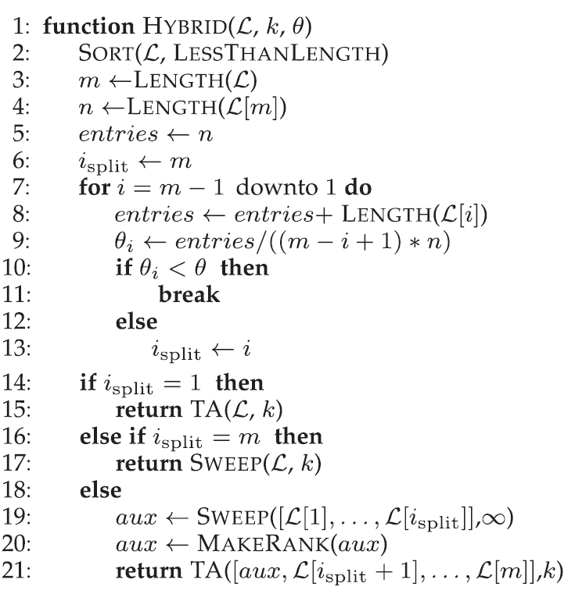
\includegraphics[width=\textwidth]{pic/hybrid.png}
        \end{column}
        \begin{column}{.7\textwidth}
            \begin{itemize}[<+->]
                \item 箱乘积中的键往往稀疏,使得 TA 算法大部分情况下需要二分查找一个不存在的键,使得TA算法并未达到实际最优。
                \item 混合算法的想法是提高箱乘积中键的密度。
                \item 长度较短的未被访问过的箱乘积,使用扫描算法,将 $k$ 取为无穷大,聚合为一个箱乘积。
                \item 与剩下的箱乘积作为阈值算法的输入,得到最终结果。
            \end{itemize}
        \end{column}
    \end{columns}
\end{frame}


\begin{frame}{实验结果}
    该论文中使用了4个数据集:
    \begin{enumerate}
        \item Wikipedia 文章编辑历史数据集,大小112M,键是文章,数量3.0M;
        \item Flickr 数据集,大小84M,键是标签,数量1.6M;
        \item GitHub 项目数据集,大小58M,键是项目,数量1.5M;
        \item Microblogs 的数据集,大小40M,键是主题标签,数量4.7M。
    \end{enumerate}
    Wikipedia 数据集的记录数最多,Microblogs 数据集拥有最多的不同的关键词。
\end{frame}

\begin{frame}{简单对比实验}
    \begin{figure}
        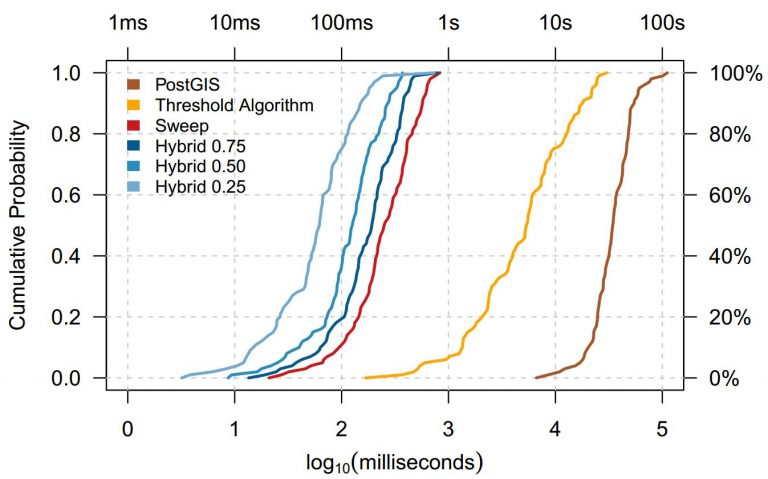
\includegraphics[width=.5\textwidth]{pic/blog.jpg}
        \caption{Microblogs 上 100 条包含时空信息的对前 32 相关的键的查询的时间效率的经验累计分布图}
    \end{figure}
\end{frame}

\begin{frame}{TopKube 基准\footnote{\url{https://github.com/laurolins/topkube_benchmark}}}
    \begin{figure}
        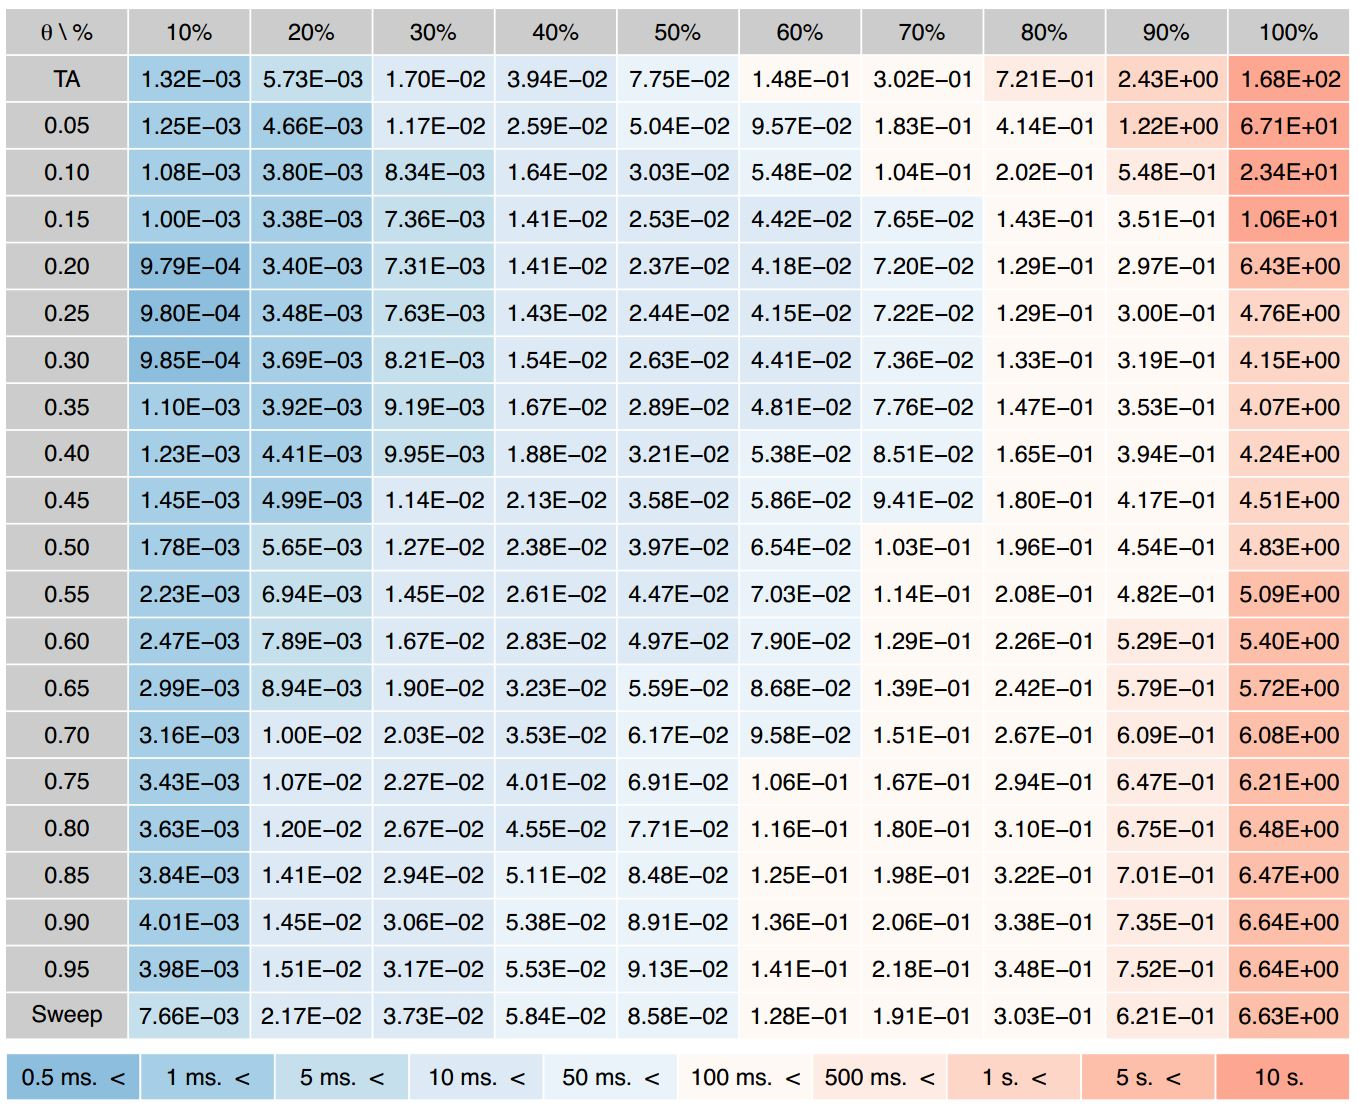
\includegraphics[width=.4\textwidth]{pic/time-peformance.jpg}
        \caption{TopKube 基准中的各算法延迟分布}
    \end{figure}
\end{frame}

\begin{frame}{加速比与 $k$ 的关系}
    当$\theta = 0.25$时,$k \leq 100$会使得算法依然能在交互性要求的时间内返回查询结果,当超过 $100$ 时,则适合使用扫描算法。

    \begin{figure}
        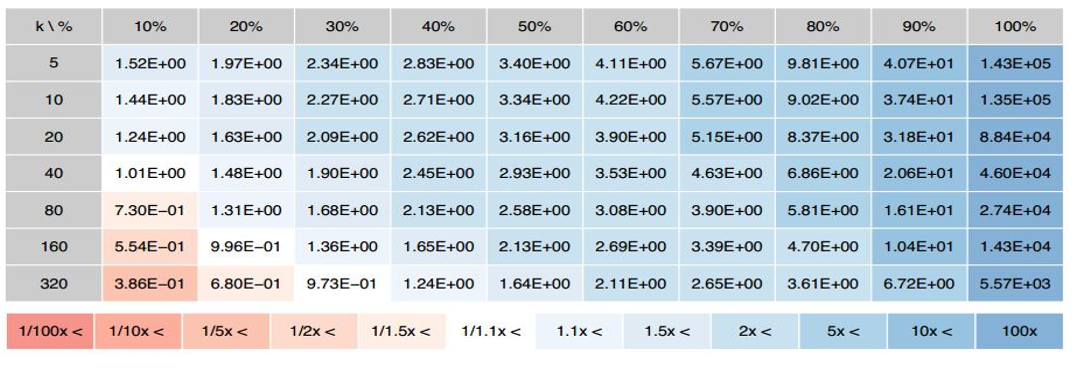
\includegraphics[width=.5\textwidth]{pic/speedup-to-sweep.png}
        \caption{阈值为0.25阈值算法和混合算法相对于扫描算法的加速比分布图}
    \end{figure}

\end{frame}

\begin{frame}{加速比与键的数量、排序数组的数量的关系}
    \begin{figure}
        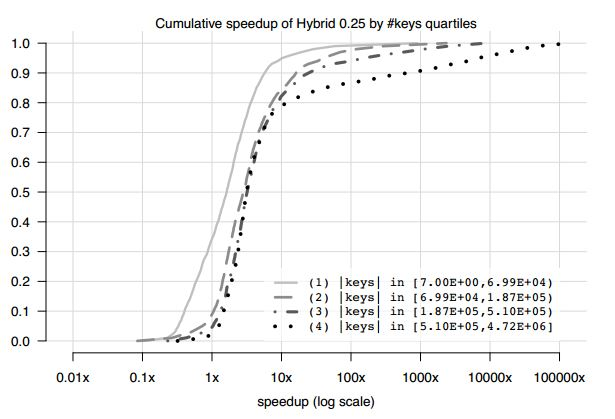
\includegraphics[width=.4\textwidth]{pic/speedup-keys.jpg}
        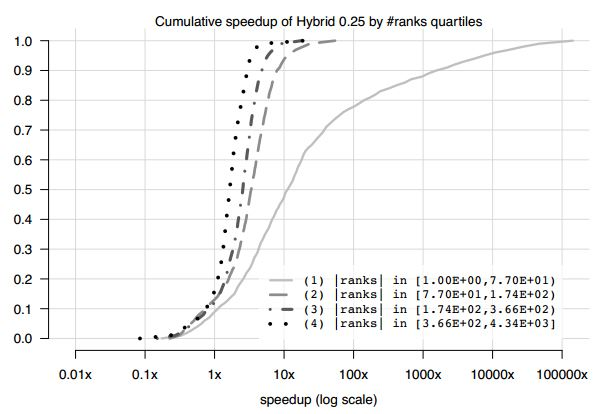
\includegraphics[width=.4\textwidth]{pic/speedup-ranks.jpg}
    \end{figure}
    \begin{itemize}
        \item 键数量越多,则 $\theta = 0.25$的混合算法加速比越高。
        \item 排序数组的数量越多,则加速比越小。
    \end{itemize}
\end{frame}

\begin{frame}{总结}
    \begin{itemize}[<+->]
        \item 通过扩展 Nanocubes,提升了的效率,使得交互式查询成为可能。
        \item 可能的改进之处:
              \begin{itemize}
                  \item 不同条件下,达到最优的 $\theta$ 值不同,如何进行自适应的 $\theta$ 选取是接下来可以进行改进之处。
                  \item 论文主要关注时间效率的提升,因此对于空间存储,没有进行特别的优化。
              \end{itemize}
    \end{itemize}

\end{frame}

\begin{frame}{参考文献}
    \printbibliography
\end{frame}

\begin{frame}
    \begin{center}
        \Huge
        谢谢聆听
    \end{center}
\end{frame}

\end{document}
